\clearpage

\begin{refsection}

\section{SNR of the Photoelectron Generator}

\begin{tcolorbox}	
\begin{tabular}{p{2.75cm} p{0.2cm} p{10.5cm}} 	
\textbf{Header File}   &:& srn\_photoelectron\_generator\_*.h \\
\textbf{Source File}   &:& snr\_photoelectron\_generator\_*.cpp \\
\textbf{Version}       &:& 20180309 (Diamantino Silva)
\end{tabular}
\end{tcolorbox}

\vspace{1em}
%
This block estimates the signal to noise ratio (SNR) of a input stream of photoelectrons, for a given time window.
%
\begin{figure}[h]
	\centering
	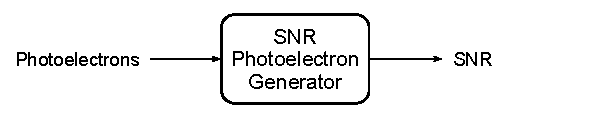
\includegraphics{./lib/snr_photoelectron_generator/figures/snr_photoelectron_generator_scheme.pdf}
	\caption{Schematic representation of the SNR of the Photoelectron Generator code block}
\end{figure}

\subsection*{Theoretical description}
%
The input of this block is a stream of samples, $y_j$, each one of them corresponding to a number of photoelectrons generated in a time interval $\Delta t$. These photoelectrons are usually the output of a photodiode (photoelectron generator).
To calculate the SNR of this stream, we will use the definition used in
\cite{saleh1991}
%
\begin{equation}
	\textrm{SNR} = \frac{\bar{n}^2}{\sigma_n^2}
\end{equation}
%
in which $\bar{n}$ is the mean value and $\sigma_n^2$ is the variance of the photon number in a given time interval $T$.
\\
To apply this definition to our input stream, we start by separate it's samples in contiguous time windows with duration $T$. Each time window $k$ is defined as the time interval $\left[ k T, (k+1) T \right[$. To estimate the SNR for each time window, we will use the following estimators for the mean, $\mu_k$, and variance, $s_k^2$
\cite{smith1997}
%
\begin{equation}
	\mu_k = \braket{y}_k
	\qquad \qquad
	s_k^2 = \frac{N}{N-1} \left( \braket{y^2}_k - \braket{y}_k^2 \right)
\end{equation}
%
were $\braket{y^n}_k$ is the $n$ moment of the $k$ window given by
%
\begin{equation}
	\braket{y^n}_k = \frac{1}{N_k} \sum_{j = j_\textrm{min}(k)}^{j_\textrm{max}(k)} y_j^n
\end{equation}
in which
\begin{align}
	j_{min}(k) &= \lceil{t_k/\Delta t \rceil}\\
	\label{eq:sample_limit_min}
	j_{max}(k) &= \lceil{t_{k+1}/\Delta t \rceil} - 1\\
	\label{eq:sample_limit_max}
	N_k &= j_{max}(k) - j_{min}(k) + 1\\
	\label{eq:n_window_samples}
	t_k &= k T
\end{align}
where $\lceil x \rceil$ is the ceiling function.\\
%
In our implementation, we define two variables, $S_1(k)$ and $S_2(k)$, corresponding to the sum of the samples and the sum of the squares of the sample in the time interval $k$.
These two sums are related to the moments as
\begin{align}
	S_1(k) &= N_k \braket{y}_k\\
	S_2(k) &= N_k \braket{y^2}_k
\end{align}
Using these two variables, we can rewrite $\mu_k$ and $s^2_k$ as
\begin{equation}
	\mu_k = \frac{S_1(k)}{N_k}
	\qquad \qquad
	s_k^2 = \frac{1}{N_k-1} \left( S_2(k) - \frac{1}{N_k}(S_1(k))^2 \right)
\end{equation}
The signal to noise ratio of the time interval $k$, $\textrm{SNR}_k$, can be expressed as
\begin{equation}
	\textrm{SNR}_k = \frac{\mu_k^2}{\sigma_k^2} =  \frac{N_k - 1}{N_k}\frac{(S_1(k))^2}{N_k S_2(k) - (S_1(k))^2}
	\label{eq:snr_estimation}
\end{equation}
%
One particularly important case is the phototelectron stream resulting from the conversion of a laser photon stream by a photodiode (photoelectron generator). The resulting SNR will be
\cite{saleh1991}
%
\begin{equation}
	\textrm{SNR} = \eta \bar{n}
	\label{eq:ideal_poisson_snr}
\end{equation}
in which $\eta$ is the photodiode quantum efficiency.
%
\subsection*{Functional description}
%
This block is designed to operate in time windows, dividing the input stream in contiguous sets of samples with a duration $\texttt{tWindow} = T$.
For each time window, the general process consists in accumulating the input sample values and the square of the input sample values, and calculating the SNR of the time window based on these two variables.\\
To process this accumulation, the block uses two state variables, \texttt{aux\_sum1} and \texttt{aux\_sum2}, which hold the accumulation of the sample values and accumulation of the square of sample values, respectively.\\
The block starts by calculating the number of samples it has to process for the current time window, using equations \ref{eq:sample_limit_min}, \ref{eq:sample_limit_max} and \ref{eq:n_window_samples}.
If the duration of \texttt{tWindow} is $0$, then we assume that this time window has infinite time (infinite samples).
The values of \texttt{aux\_sum1} and \texttt{aux\_sum2} are set to $0$, and the processing of the samples of current window begins.\\
After processing all the samples of the time window, we obtain $S1(k)$ and $S2(k)$ from the state variables as $S1(k) = \texttt{aux\_sum1}$ and $S_2(k) = \texttt{aux\_sum2}$, and proceed to the calculation of the $\textrm{SNR}_k$, using equation \ref{eq:snr_estimation}.\\
If the simulation ends before reaching the end of the current time window, we calculate the $\textrm{SNR}_k$, using the current values of \texttt{aux\_sum1}, \texttt{aux\_sum2} for $S_1(k)$ and $S_2(k)$, and the number of samples already processed, $\texttt{currentWindowSample}$, for $N_k$.
%
%
%
%
\subsection*{Input Parameters}

\begin{table}[H]
	\centering
	\begin{tabular}{|c|c|c|}
		\hline
		\textbf{Parameter}	& \textbf{Default Value}	& \textbf{Description} \\
		\hline
		windowTime			& 0							& SNR time window. \\
		\hline
		%confidenceInterval	& 0.9						& Output SNR confidence interval. \\
		%\hline
	\end{tabular}
\end{table}




\subsection*{Methods}

SnrPhotoelectronGenerator() {}
\bigbreak
SnrPhotoelectronGenerator(vector$<$Signal *$>$ \&InputSig, vector$<$Signal *$>$ \&OutputSig) :Block(InputSig, OutputSig) {}
\bigbreak
void initialize(void)
\bigbreak
bool runBlock(void)
\bigbreak
void setTimeWindow(\texttt{t\_real} timeWindow)
%\bigbreak
%void setConfidenceInterval(\texttt{t\_real} confidenceInterval)
%
%
%
%
\pagebreak

\subsection*{Input Signals}

\subparagraph*{Number:} 1

\subparagraph*{Type:} Electrical (TimeDiscreteAmplitudeContinuousReal)

\subsection*{Output Signals}

\subparagraph*{Number:} 1

\subparagraph*{Type:} Electrical (TimeDiscreteAmplitudeContinuousReal)

\subsection*{Examples}

\begin{figure}[h]
	\centering
	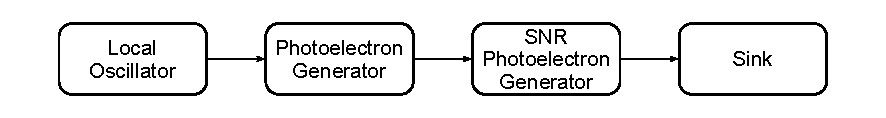
\includegraphics[width=\textwidth]{./lib/snr_photoelectron_generator/figures/scheme-simulation.pdf}
	\caption{Simulation setup}
\end{figure}

To confirm the block's correct output, we have designed a simulation setup which calculates the SNR of a stream of photoelectrons generated by the detection of a laser photon stream by a photodiode.\\
The simulation has three main parameters, the power of the local oscillator, $P_{LO}$, the duration of the time window, $T$, and the photodiode's quantum efficiency, $\eta$. For each combination of these three parameters, the simulation generates $1000$ SNR samples, during which all parameters stay constant.
The final result is the average of these SNR samples.\\
The simulations were performed with a sample time $\Delta t = 10^{-10} s$.
%
\begin{figure}[H]
	\centering
	\begin{subfigure}{0.45\textwidth}
		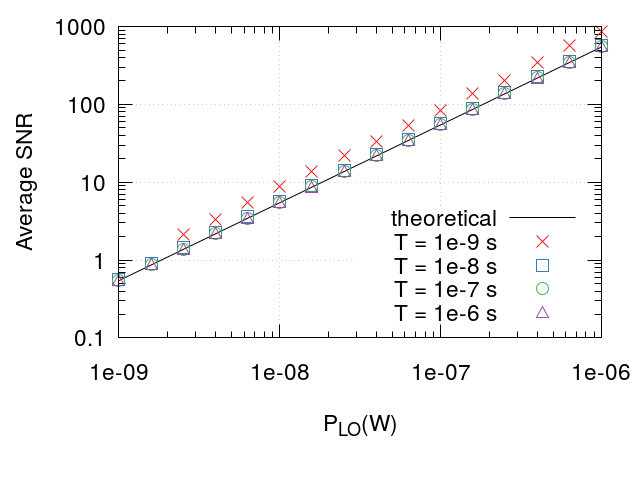
\includegraphics[width=\textwidth]{./lib/snr_photoelectron_generator/figures/plot-snr-eff-0_7.png}
		\caption{$\eta = 0.7$}
		\label{pl:sim-results-07}
	\end{subfigure}
	\hspace{10mm}
	\begin{subfigure}{0.45\textwidth}
		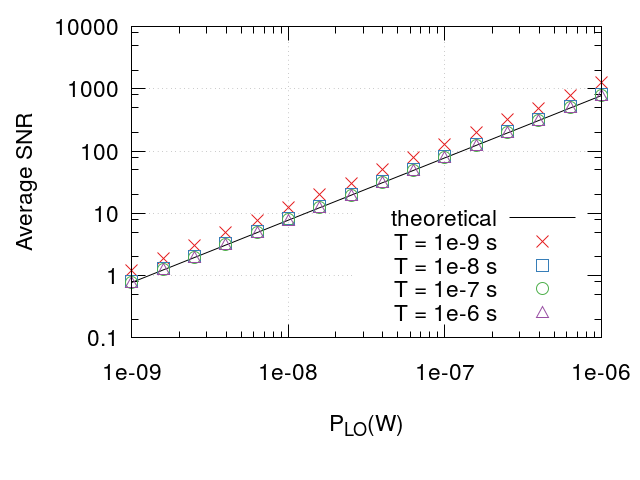
\includegraphics[width=\textwidth]{./lib/snr_photoelectron_generator/figures/plot-snr-eff-1.png}
		\caption{$\eta = 1$}
	\end{subfigure}
	\caption{Theoretical and simulated results of the average SNR, for two photodiode efficiencies.}
	\label{pl:sim-results}
\end{figure}
%
The plots in \ref{pl:sim-results} show the comparison between the theoretical result \ref{eq:ideal_poisson_snr} and the simulation results.
We see that for low values of $T$, the average SNR shows a systematic deviation form the theoretical resul, but for $T > 10^{-6}s$ ($10000$ samples per time window), the simulation result shows a very good agreement with the theoretical result.\\
\\
The simulations also show a lack of average SNR results when low power, low efficiency and small time window are combined (see plot \ref{pl:sim-results-07}). This is because in those conditions, the probability of having a time windows with no photoelectrons, creating a invalid SNR, is very high, which will prevent the calculation of the average SNR.\\
We can estimate the probability of calculating a valid SNR average by calculating the probability of no time window having $0$ phototelectrons, $p_{ave} = (1-q)^M$, in which $q$ is the probability of a time window having all it's samples equal to $0$ and $M$ is the number of time windows.
We know that the input stream follows a Poisson distribution with mean $\bar{m}$, therefore $q = (\exp (- \bar{m}))^N$, in which $\bar{m} = \eta P \lambda /h c$ and $N = T/\Delta t$, is the average number of samples per time window.
Using this result, we obtain the probability of calculating a valid SNR average as
\begin{equation}
	p_{ave} = \left( 1 - \exp( - N \bar{m}) \right)^M
\end{equation}



\subsection*{Block problems}




\subsection*{Future work}

The block could also output a confidence interval for the calculated SNR.
Given that the output of the Photoelectron Generator follows a Poissonian distribuition when the shot noise is on, the article "Confidence intervals for signal to noise ratio of a Poisson distribution" by Florence George and B.M. Kibria \cite{george2011}, could be used as a reference to implement such feature.



% bibliographic references for the section ----------------------------
\clearpage
\printbibliography[heading=subbibliography]
\end{refsection}
\addcontentsline{toc}{subsection}{Bibliography}
\cleardoublepage
% --------------------------------------------------------------------- 
